\documentclass[preprintnumbers,amsmath,amssymb,superscriptaddress,twocolumn,showpacs]{revtex4-2}
\usepackage{graphicx}% Include figure files
\usepackage{dcolumn}% Align table columns on decimal point
\usepackage{bm}% bold math
\usepackage{natbib}
\usepackage{physics}
\usepackage[caption=false]{subfig}



%\newcommand{|}{Y$_2$SiO$_5$}
\def\sgn{\mathop{\rm sgn}}
\newcommand{\be}{\begin{equation}}
\newcommand{\ee}{\end{equation}}
\newcommand{\bea}{\begin{eqnarray}}
\newcommand{\eea}{\end{eqnarray}}

\begin{document}

\title{Depolarization of Interacting NV ensembles : \\
The Role of Local Electric Fields and Double Flip processes}

\author{C. Pellet-Mary$^1$, M. Perdriat$^1$, P. Huillery$^?$,  G. H\'etet} 

\affiliation{Laboratoire De Physique de l'\'Ecole Normale Sup\'erieure, \'Ecole Normale Sup\'erieure, PSL Research University, CNRS, Sorbonne Universit\'e, Universit\'e Paris Cit\'e , 24 rue Lhomond, 75231 Paris Cedex 05, France.}

\begin{abstract}
We present experimental results on dipolar interaction processes in ensemble of spin-1 systems. Using the spin of highly doped ensembles of negatively charged nitrogen vacancy centers in diamonds, we identify regimes where flip-flop, double-flip processes as well as the mixing induced by local electric field dominate.
%We analyse these results from the perspective of magnetometry applications, and show that both double-flip processes and local electric fields improve the magnetic field sensitivity.
Our results are relevant for understanding decoherence in many-body spin systems as well as for high sensitivity magneto- and electro-metry with long-lived interacting solid-state spins. As a proof of principle, we present an orientation-free and microwave-free magnetometer operating with a sensitivity below $100$ nT/$\sqrt{\rm Hz}$.
\end{abstract}

\maketitle

%\begin{figure}
%\includegraphics[width=0.45\textwidth]{Figures/fig_dense_vs_pas_dense.pdf}
%\caption{Photoluminescence measurement from NV centers ensemble as a function of an external magnetic field applied in an arbitrary direction (a) for a CVD sample containing $\approx$ 4 ppb NV$^-$ centers, (b) for an HPHT sample containing $\approx$ 3 ppm NV$^-$ centers}
%\label{PL_NV_density}
%\end{figure}

%In this letter/article, we characterize the depolarization of the spins observed for dense ensemble of NV centers in zero magnetic field and its potential application for DC magnetometry. While the main mechanism behind the depolarization, the lift in the degeneracy between the four classes of NV centers, is already well studied and can be exploited in a microwave-less vector magnetometry protocol, we found two other depolarization mechanisms specific to the zero-field region which could play an important role in a low-field magnetometry protocol.
%
%The main signature of the spin depolarization in low field is the characteristic dip in photoluminescence (PL) observed only for high density ($\gtrsim 1$ ppm) of NV centers, as shown on fig \ref{PL_NV_density}. The decrease in the spins' lifetime in zero field makes the optical polarization scheme of the NV centers less effective and therefore reduce the population of the bright $\ket{0}$ spin state. %The reason for the decrease in PL at higher magnetic field values is the mixing of the bright spin state $\ket{0}$ to the darker state $\ket{-1}$ induced by the transverse magnetic field. This effect does not modify (on first approximation) the spins' lifetime, and is common to both dense and sparse samples.

The electronic spin properties of the negatively charged nitrogen-vacancy (NV$^-$) center in diamond has given rise to a wealth of applications in nanoscale sensing and quantum information science in part thanks to the possibility to optically polarize and read-out its spin state at ambient conditions. Many recent work indeed focus on ensembles of spins from NV centers with the prospect to boost the magnetic field sensing capabilities and for studying many body effects
\citep{TALLAIRE2020421,edmonds2021characterisation, chatzidrosos2021fiberized, kucsko2018critical, giri_coupled_2018}

When the spin ensemble becomes dense, inhomogeneities in the relaxation rates of NVs can give rise to spin depolarisation with a very rich many body dynamics associated with disorder \citep{choi_observation_2017}. This mechanisms however limits the efficiency of magnetometers \citep{zhou2020quantum}
%It was proposed to exploit these CR to perform sensitive microwave free magnetometry (REF).  
Recent magnetometry proposals have been put forward at zero magnetic field. There, the depolarisation effect was shown to be much stronger, but the detailed studies of relaxation mechanisms have not been identified to the best of our knowledge. Some of the possible processes that lead to cross-relaxation in strongly coupled dipolar systems are depicted in Fig.~1. The goal of this paper is to identify regimes where the spin flip-flop within different classes of NV centers, double-flip up and down as well as the mixing induced by local electric field play a role. 

The electronic spin of NV center is a spin-1 system in the ground state (see Fig. 1). It can be optically polarized in the $\ket{m_s=0}$ state. The photoluminescence of this state is also is larger than the $\ket{m_s=\pm 1}$ states enabling spin-read out at ambient temperature. The $\ket{m_s=\pm 1}$ spin states are separated from the $\ket{m_s=0}$ state by  $D = (2\pi) 2.87$ GHz so that when a resonant microwave or static transverse magnetic field is applied, the photoluminescence is reduced \citep{epstein2005anisotropic,lai2009influence}. 
Fig.  \ref{T1}-a) and b) show the change in photoluminescence (PL) with respect to an external magnetic field for two samples with a low and high concentration of NV$^-$ centers (see SI). Both samples show a decrease in PL as the magnetic field amplitude increases.  There is however a stark difference in the low magnetic field region where only high-density samples shows a drop in PL \citep{jarmola_longitudinal_2015,  mrozek_longitudinal_2015}. This effect can be observed on all our samples (see SI) whenever the NV concentration lies in the ppm range. The drop of the PL at low magnetic field is associated with a decrease of the NV's spin lifetime $T_1$ \citep{jarmola_temperature-_2012}, which results in a decrease of the population in the bright state $\ket{0}$.

%Indeed, since the $\ket{m_s=0}$ spin state is brighter than the $\ket{m_s=\pm 1}$ states, and since the optical pumping in the $\ket{m_s=0}$ state is in competition with the relaxation in a thermal distribution of the states, decreasing the spins lifetime results in a decrease of the NV PL \citep{finco2021imaging}.
%To understand the behavior of the PL in zero-field, we therefore need to study the dynamics of the spin in the low magnetic field region.
The depolarization dynamics of the spin of single or dilute NV centers at room temperature is dominated by two-phonon Raman processes \citep{redman1991spin,jarmola_temperature-_2012,norambuena2018spin}, which depend on the crystal lattice temperature. It has been observed that dense NV centers ensemble have an additional spin decay channel \citep{jarmola_temperature-_2012,jarmola_longitudinal_2015,mrozek_longitudinal_2015, choi2017depolarization, akhmedzhanov_microwave-free_2017, akhmedzhanov_magnetometry_2019, pellet2021magnetic, mrozek2021characterization}, which depends greatly on the magnetic field amplitude. This effect has been attributed to cross-relaxation between the NV centers through dipole-dipole coupling \citep{mrozek_longitudinal_2015, choi2017depolarization}.  Inhomogeneity of the spin lifetimes is further needed in order to explain the depolarization of the spin ensemble \citep{choi2017depolarization}. We will denote $T_1^{\rm ph}$ the characteristic timescale associated with the phonon relaxation process and $T_1^{\rm dd}$ the density dependent timescale associated with the dipole-dipole relaxation process.

\begin{figure}
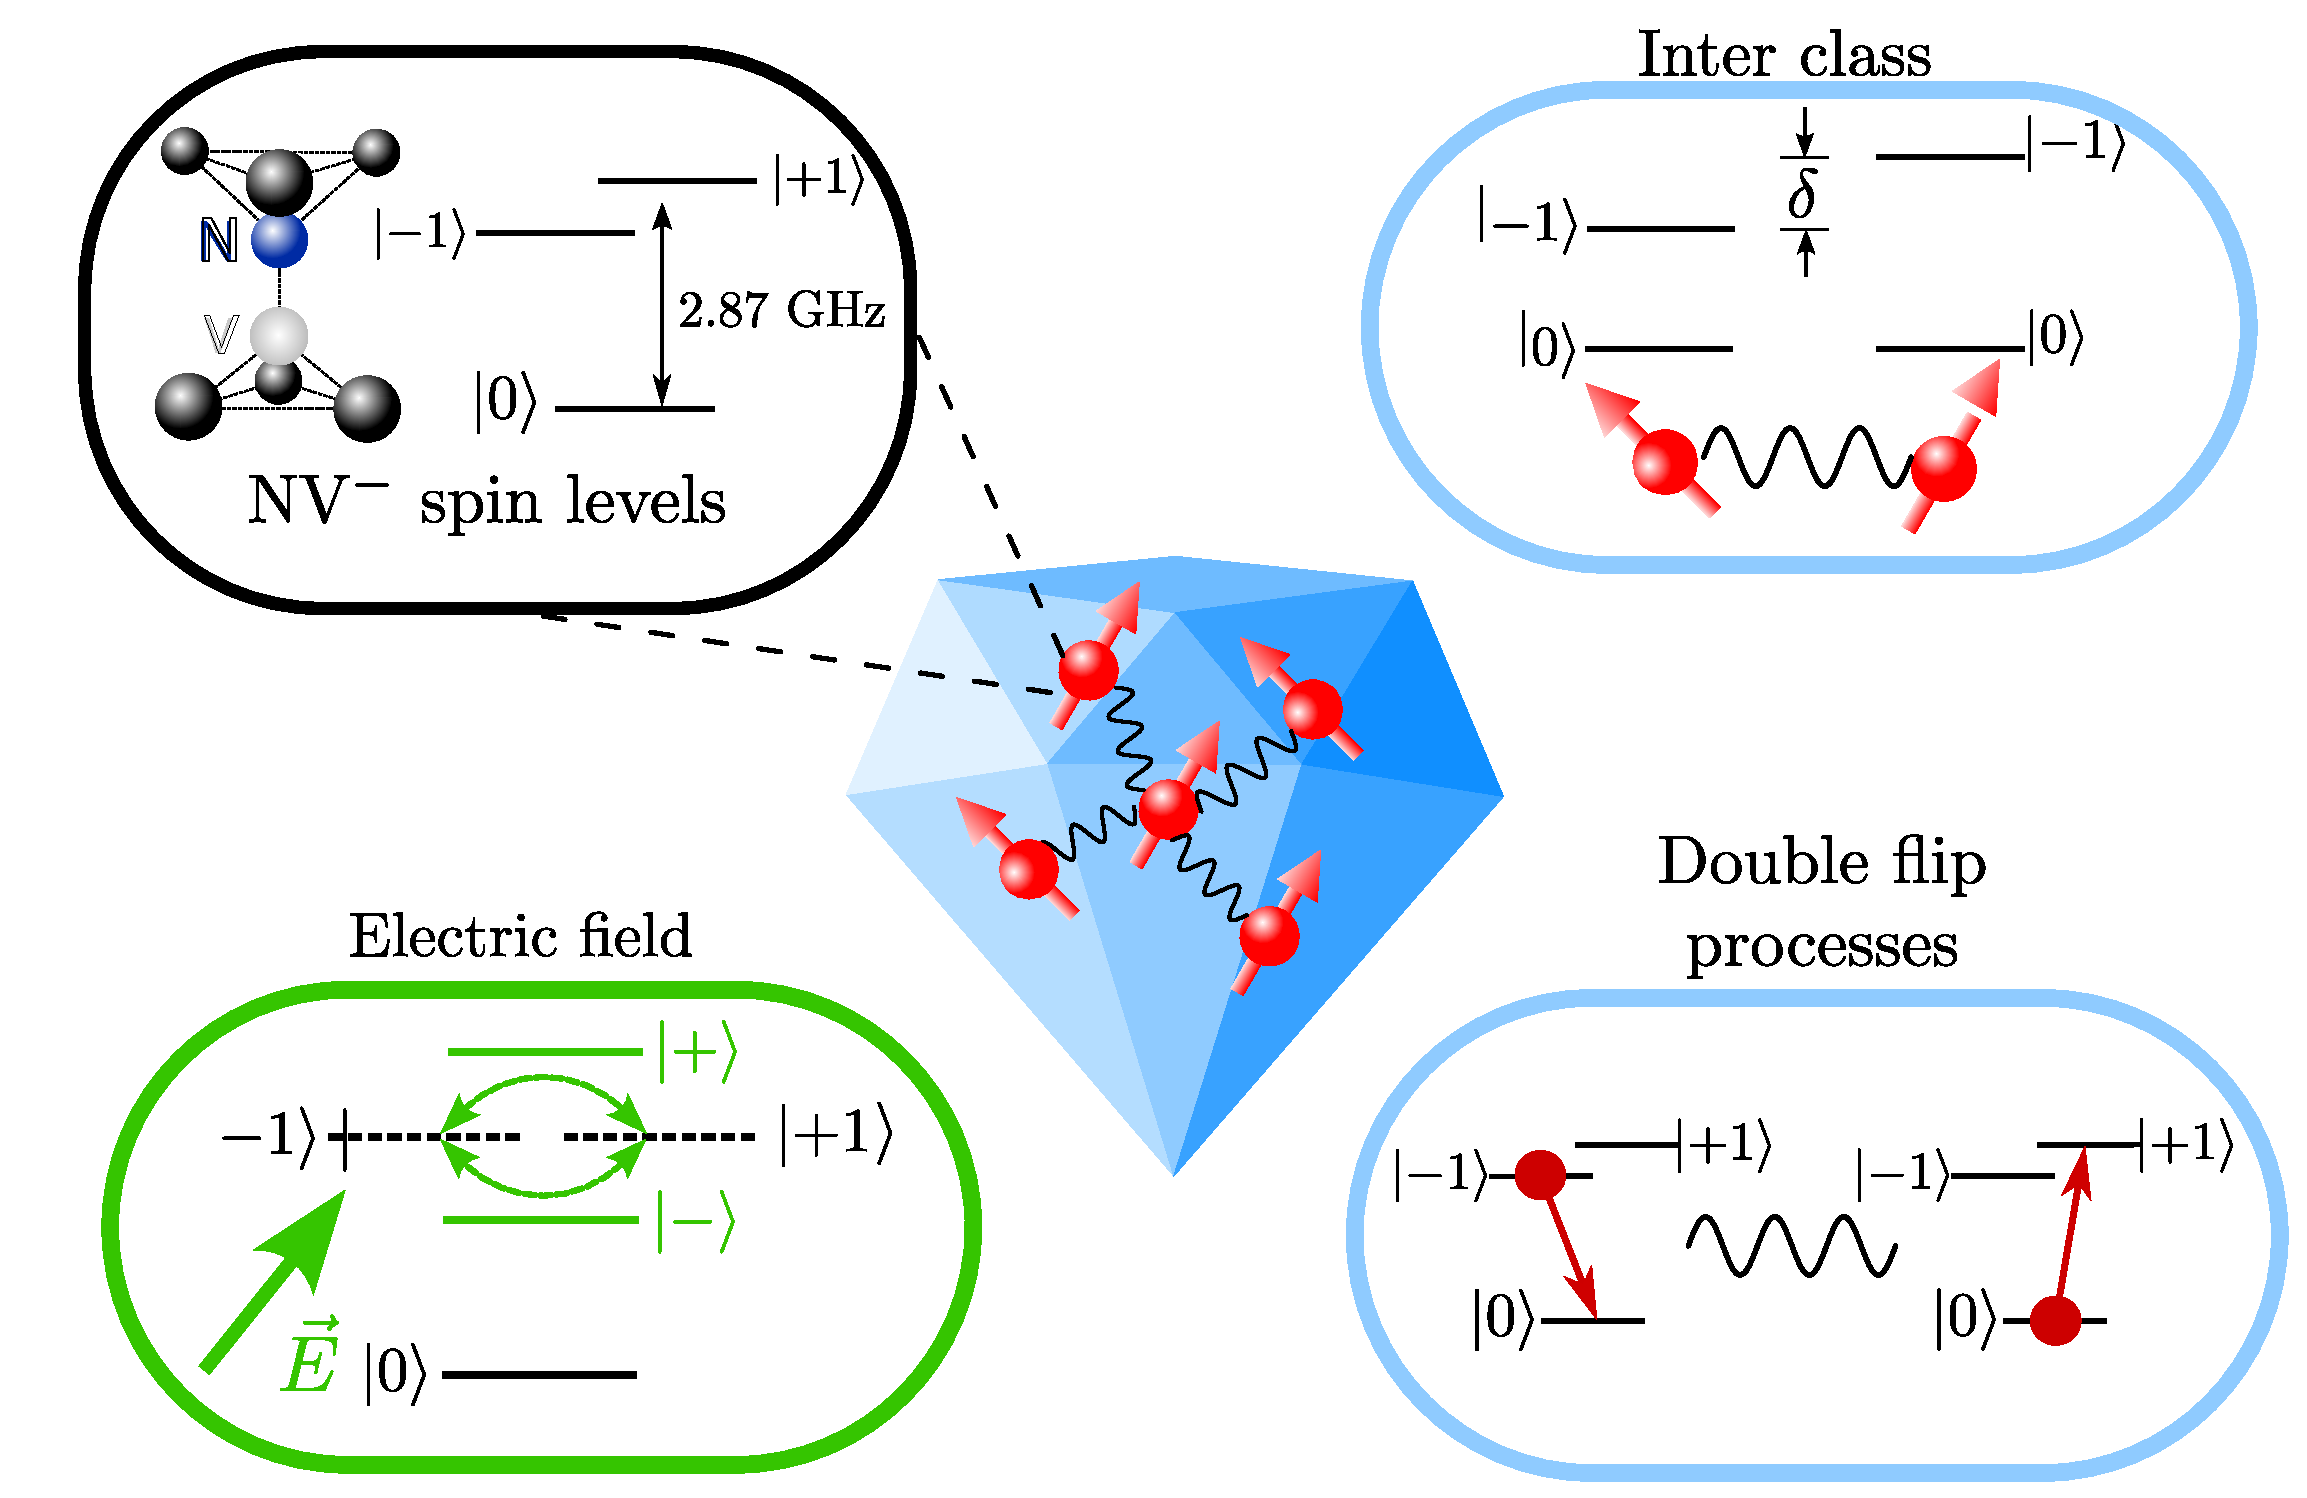
\includegraphics[width=0.45\textwidth]{Figures/shema_summary.pdf}
\caption{Schematics showing a diamond with interacting spins as well as the three processes that can account for dipolar relaxation. }
\label{schema_intro}
\end{figure}

\begin{figure}
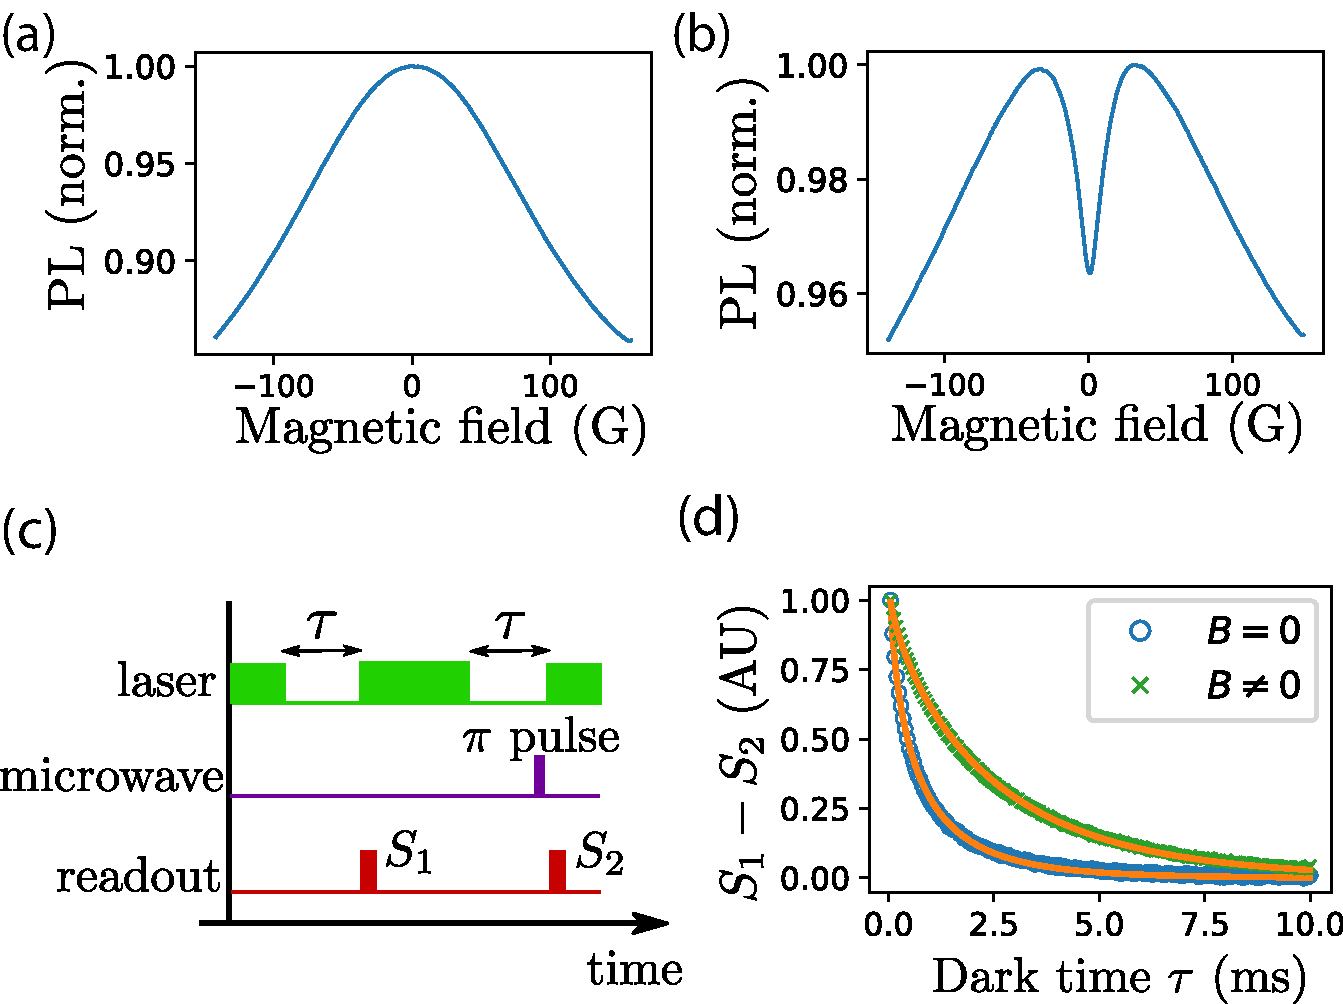
\includegraphics[width=0.45\textwidth]{Figures/fig_T1.pdf}
\caption{a) Photoluminescence measurement from NV centers ensemble as a function of an external magnetic field applied in an arbitrary direction (a) for the sample CVD-PPB, with [NV$^-$]$\approx 50\ \rm ppb$ (b) for the sample HPHT-150-1, with [NV$^-$]$\approx 3\ \rm ppm$. (c) Sequence used to measure the spin lifetime. (d) Spin relaxation $S_1-S_2$ measured for the dense sample at zero and non-zero magnetic fields. The fitting procedure (orange plain line) is detailed in the main text}
\label{T1}
\end{figure}

\begin{figure*}
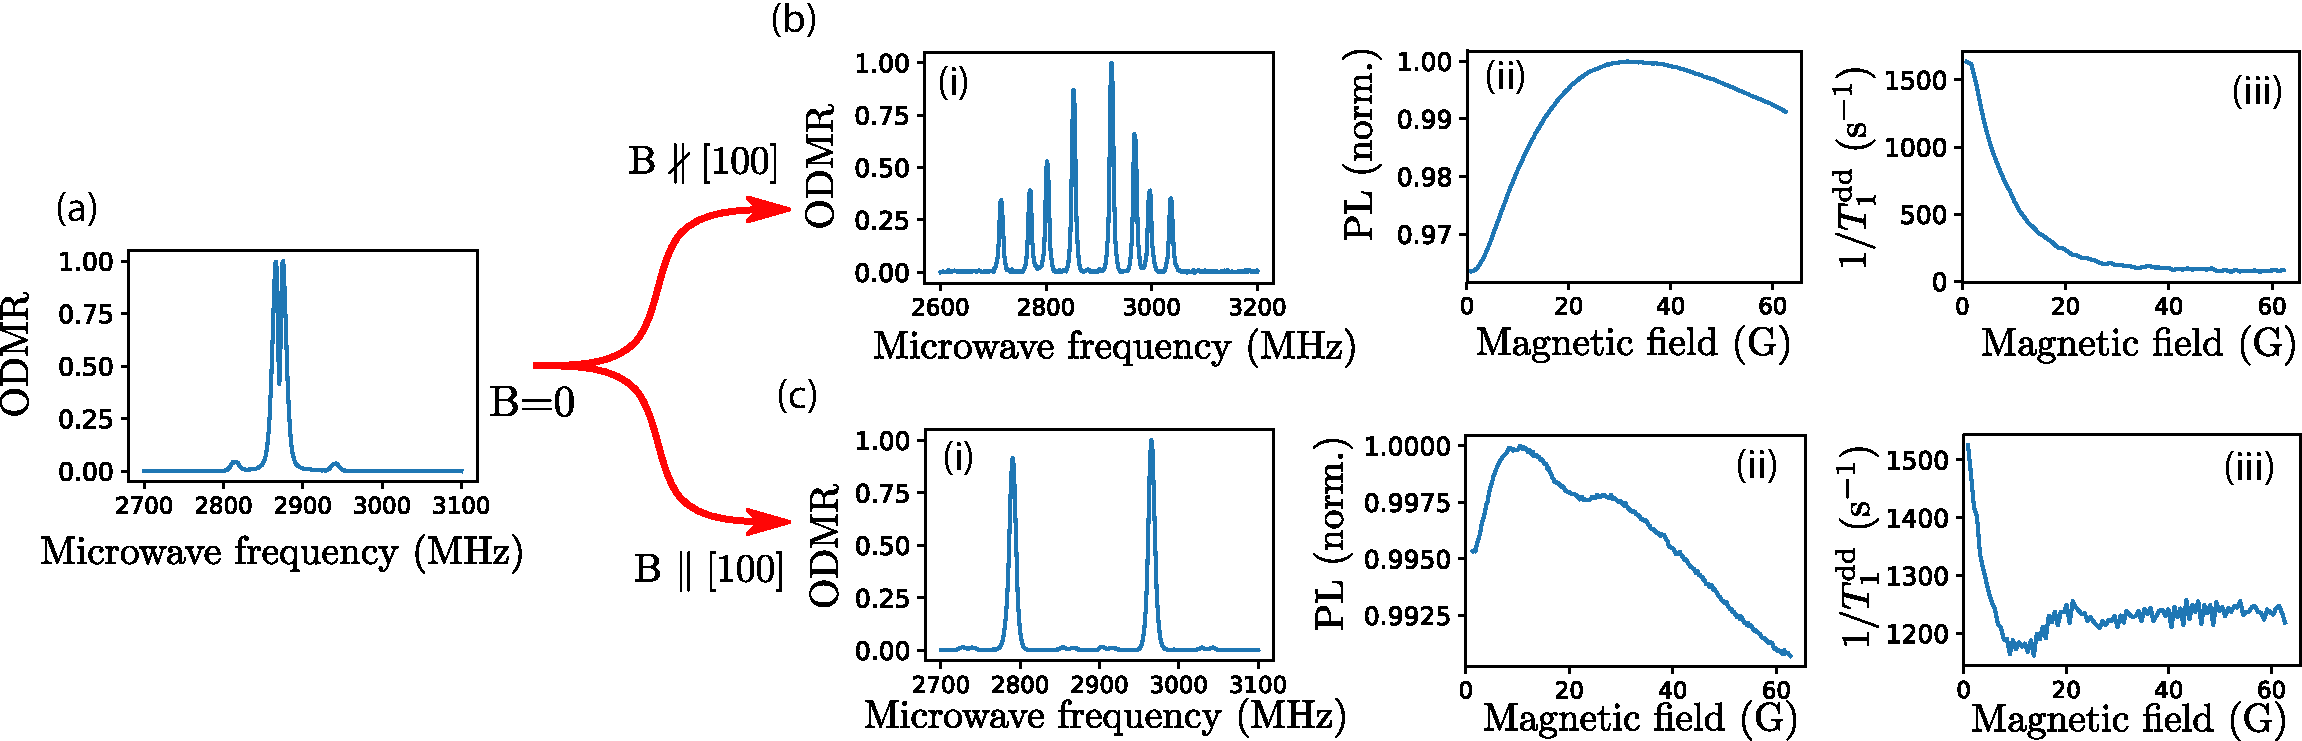
\includegraphics[width=.95\textwidth]{Figures/fig_100_vs_1x1x1x1.pdf}
\caption{(a) ODMR spectrum in zero field. (b)-i) ODMR spectrum for a magnetic field $\approx$ 60 G, misaligned by $\sim  24^\circ$ from the [100] axis. (b)-ii) Normalized photoluminescence of the NV$^-$ ensemble as a function of the magnetic field amplitude. (b)-iii) Stretched part of the spin decay $1/T_1^{\rm dd}$ as a function of the magnetic field amplitude. (c)-i), (c)-ii) and (c)-iii) : same measurements but with a magnetic field close to the [100] axis}
\label{100_VS_1x4}
\end{figure*}

Fig. \ref{T1}-c) shows the sequence employed for measuring $T_1^{\rm dd}$ in the dense sample. 
%The spin lifetime protocol used here is described in Fig. \ref{T1} and is based on previous similar experiments 
It consists in a pump-probe measurement where the spins are first polarized in the $\ket{0}$ state by a green laser, and read-out optically after a variable dark time $\tau$. In highly doped samples, this sequence often results in artifacts, mostly due to charge state transfer in the dark \citep{giri_coupled_2018, giri_selective_2019}. It is therefore convenient to repeat the sequence with an additional $\pi$ pulse right before the spin read-out to prepare the remaining $\ket{0}$ polarization into a darker $\ket{+1}$ or $\ket{-1}$ state. By subtracting the result of the two sequences, we select only the spin-dependent part of the signal, with the added benefit of being able to select a specific class of NV centers \citep{jarmola_temperature-_2012, mrozek_longitudinal_2015, choi2017depolarization}. 

Fig. \ref{T1}-b) shows the subtracted signals when $B\approx 0$ and $B \approx 50\ \rm G$.
The ensemble spin decay curves are not exponential, which was found to be due to inhomogeneities between the spin lifetimes of dipolar coupled NV$^-$ centers \citep{choi2017depolarization}.
We will base our interpretations of the experimental results on the NV-fluctuator model developed in \citep{choi2017depolarization}. This model postulates the existence of very short-lived NV centers - the so-called fluctuators - which, when coupled resonantly to the other NV centers, act as a sink of polarization for the spin ensemble. A conclusion of this model is that, for a homogeneous 3D distribution of fluctuators, the dipole-induced lifetime should be stretched-exponential with a stretch factor $\beta=1/2$. Such an ensemble lifetime is indeed observed when $T_1^{\rm dd} \ll T_1^{\rm ph}$.
For the samples used in this paper (detailed in SI) $T_1^{\rm dd} \sim T_1^{\rm ph}$, so both decay processes have to be included in the analysis. Fitting the two curves by the product of an exponential and a stretched exponential, we find $T_1^{\rm ph}=3.6$ ms for both and $T_1^{\rm dd}= 0.6\ \rm ms$ and $13.0\ \rm ms$ respectively. We also conducted further measurements that confirm the lifetime-limited character of the fluctuator employed in the model \citep{choi2017depolarization}, see SI. 
%These results show that our sample clearly manifests dipolar interactions amongst closely packed NV centers, but do not tell about the magnitude of the several possible mechanisms involved in the dipolar relaxation. 
%In spin-1 systems, there can indeed be several channels for decay at zero fields such as flip-flop, double flip, 

%The resulting fitting formula is therefore :
%\begin{equation}
%S(\tau)=A \exp (-\frac{\tau}{T_1^{\rm ph}} -\sqrt{\frac{\tau}{T_1^{\rm dd}}}),
%\end{equation}
%Further details on the fitting procedure are available in SI. For the rest of the article we will be only interested on the stretched exponential lifetime ${T_1^{\rm dd}}$.

One of the ways to tune dipole-dipole related phenomena is by changing the number of resonant spins. Fig. \ref{100_VS_1x4} (b)-i) shows an optically detected magnetic resonance (ODMR) spectrum from the dense ensemble HPHT-150-1. The observed lines correspond to the projections of the magnetic fields onto the four "classes" of NV centers - that is physical orientation of the NV axis is the diamond crystal cell - together with the two possible spin transitions $\ket{0}\to\ket{-1}$ and $\ket{0}\to\ket{+1}$. The transitions frequencies of the four different classes can be controlled by changing the amplitude and orientation of the external magnetic field. Fig. \ref{100_VS_1x4} (c)-i) shows an example where all four classes are brought to resonance by placing the magnetic field along the [100] crystalline axis. 
%Other example of class resonances are given in the SI.
This configuration will be essential to decipher what dipolar relaxation mechanisms play a role at low field. 

Fig. \ref{100_VS_1x4} (b)-ii) and (b)-iii) show the PL from an ensemble of NV centers as a function of the amplitude of a magnetic field aligned as in Fig. \ref{100_VS_1x4} (b)-i). 
We also extract the stretched exponential spin decay time $T_1^{\rm dd}$ by running the sequence shown in Fig. 2-c) at each of the 0.5 G magnetic field values. 
We observe that the 3 \% increase in PL under low magnetic field is indeed correlated with a drop in the spin decay rate from 1.6 kHz to 0.08 kHz, as the magnetic field increases. This result can be explained by the higher number of resonant spins in zero magnetic field, where all four classes are degenerate, as opposed to $\bm B \neq 0$. The half width of the dip ($\approx 10$G) is consistent with a fluctuator model taking into account the change in the spin resonance overlaps as the $B$ field is swept (see SI).
Note that the decrease in PL for $B>40\ \rm G$ is related to state mixing by the transverse magnetic field, so it is not correlated to a modification of the spin lifetime. 

Importantly, we observed that the lifted degeneracy of the four NV classes is not the sole reason for the increase of the spin lifetime as the B field increases. Fig. \ref{100_VS_1x4} (c)-ii) and (c)-iii) show the change in the PL and in $1/T_1^{\rm dd}$ as a function of a magnetic field that is aligned along the [100] axis. For this particular orientation, the four classes are always resonant, regardless of the field amplitude. We can see that there still is an increase in the spin decay rate and a corresponding drop in the PL under low magnetic field values, although considerably reduced. 
%Also, the rate of change in both the PL and $T_1^{\rm dd}$ is larger by more than a factor of 3 in the [100] configuration. Although the contrast is smaller, this effect can thus drastically impact zero-field magnetometry protocols based on CR. C'est faux ça, c'est meme plutot le contraire ici
The main aim of this paper is to understand the physics governing the contribution to the spin decay in this second scenario. Note that the slight drop in PL and the corresponding bump for $1/T_1^{\rm dd}$ at $B \sim 20$G is related to dipolar interaction with NV centers that have a $^{13}$C as a first neighbor \cite{pellet2021optical}. 

We identified and isolated two additional mechanisms that could explain this effect : local electric fields and double-flip processes. 
The dipole-dipole interaction Hamiltonian between two spins ${\vec S}_1$ and ${\vec S}_2$ reads :
\begin{equation}
\mathcal{H}^{\rm dd}= -\frac{J_0}{r^3}\left(3\left({\vec S}_1 \cdot \vec u \right)\left({\vec S}_2 \cdot \vec u \right) - {\vec S}_1 \cdot {\vec S}_2  \right),
\end{equation}
Where $J_0= (2 \pi) 52\ \rm MHz \cdot \rm{nm}^3$, $\vec r$ is the relative positions of the two spins and $\vec u = \frac{\vec r}{\norm{\vec r}}$. In situations such as the one described in Fig. \ref{100_VS_1x4} (c)(i), the only relevant terms of $\mathcal{H}^{\rm dd}$ in terms of population transfer are the flip-flop terms such as $\mel{0,+1}{\mathcal{H}^{\rm dd}}{+1,0}$. In zero magnetic field however, we have to take into account these two other mechanisms of the dipolar Hamiltonian in consideration.
%where both NV spins involved in the dipole-dipole coupling flip their spin in the same direction.
It was shown in  \cite{mittiga2018imaging} that local electric fields coming from charge traps such as $P_1^+$ and NV$^-$ centers are responsible for the optically detected spin resonance profile at zero magnetic field in large NV ensembles. Magnetic field noise comes in to second order in zero field. %We also do not take into account the hyper-fine structure of the NV center due to the large inhomogeneous broadening of the ESR transitions (see SI). 
We will then consider the following spin Hamiltonian for the electric field dependent NV$^-$ ground state : 
\begin{equation}
\label{NV Hamiltonian}
\mathcal{H}_{\rm elec}= d_\perp \left[ E_x(S_y^2-S_x^2) + E_y(S_xS_y+S_yS_x) \right]
\end{equation}
where $E_{x,y}$ are the projections of local electric fields on the NV axes. 
Under local electric fields with orientations given by the angle $\phi_E={\rm tan}(E_x/E_y)$, the eigenstates of $H_{NV}$ are $\ket{0}$ and $\ket{\pm}=\frac{1}{\sqrt{2}}(\ket{+1}\pm e^{-i\phi_E}\ket{-1})$.
Computing the flip-flop terms $\ket{\pm,0} \bra{0,\pm} $ in the fluctuator model shows that $1/T_1^{dd}$ should be increased at zero field, even after averaging over all possible orientations $\phi_E$ (see SI).  Another mechanism at stake when considering dipolar interactions with spin-1 systems are double-flip processes. 
These processes correspond to terms like $\ket{+1,0} \bra{0,-1}$ in the anisotropic [RQ CLEMENT : pourquoi anisotropic ?] dipolar interaction, giving rise to an exchange of two units of spin-angular momentum. These processes can become significant when the states $\pm 1$ are degenerate and are thus likely to explain part of the zero-field dip in Fig. c)-ii). 
%Theoretical model predicts a factor of $\approx $5 increase in $1/T_1^{dd}$ at zero field.

In order to discriminate the role of these two effects in the low-field region, we performed another similar study under a purely transverse magnetic field.
This regime in fact emulates the effect of the electric field while turning off the resonance condition for double flip processes : indeed for relatively weak transverse magnetic field, the eigen-basis of the spin Hamiltonian is close to $\ket{0},\ket{+},\ket{-}$. This property has been used to observe a linear dependence in the electric field for the spin transition frequencies by applying an external transverse magnetic field \cite{dolde2011electric,qiu2022nanoscale}.
Fig.~\ref{B_transverse} (a) shows the energy levels for the three eigenstates of the NV spin Hamiltonian as a function of a purely transverse magnetic field. We will denote these eigenstates in the general case $\ket{g}$, $\ket{d}$ and $\ket{e}$. For weak transverse magnetic field, $\ket{g} \approx \ket{0}$, $\ket{d}=\ket{-}$ and $\ket{e} \approx \ket{+}$. As the magnetic field increases, $\ket{g}$ and $\ket{e}$ starts to become a mixing of $\ket{0}$ and $\ket{+}$ while $\ket{d}$ remains equal to $\ket{-}$.

Crucially, mixing remains even when the associated energy splitting of the $\ket{d}$ and $\ket{e}$ states is large : Fig. \ref{B_transverse}-(b) shows both the splitting between the energy levels of $\ket{d}$ and $\ket{e}$, and the matching factor $\abs{\bra{e}\ket{+}}^2$ characterizing the closeness of the states $\bra{e}$ and $\bra{+}$. We can see that at a field value of $\sim 130$ G, the splitting between the $\ket{d}$ and $\ket{e}$ reaches $\sim 50$ MHz, far exceeding the range of the dipole-dipole resonant coupling (see details in SI), but $\abs{\bra{e}\ket{+}}^2 > 0.98$ meaning that the spin Hamiltonian eigenstates are still roughly in the $\ket{0}, \ket{+}, \ket{-}$ basis. We can therefore decouple the effects of the double-flip processes  $\propto \ket{g,d}\bra{d,e}$, which are no longer resonant when $| \bm B | \geq 100$ G, from the effects of the mixing induced by the transverse electric - or in this case magnetic - field.

Fig. \ref{B_transverse}-(c) shows the measurement of the stretched lifetime $T_1^{\rm dd}$ for a single class of NV centers exposed to a transverse magnetic field between 20 and 130 G on another sample HPHT-150-2, upon which we measured a stretched decay $1/T_1^{\rm dd}=25\pm 5\  \rm Hz$ in the case of strong longitudinal magnetic field. The detuning $\Delta \nu$ between the two states $\ket{d}$ and $\ket{e}$ was measured through ODMR. We attribute the decrease in the spin decay rate when the detuning increases to the loss of effectiveness of the double-flip processes. We can notice that the decay rate reaches a plateau for $\Delta \nu \geq 30\ \rm MHz$ with a value $1/T_1^{\rm dd}=57\pm 5\  \rm Hz$ about twice as large as the decay rate for a longitudinal magnetic field. This plateau we attribute to the effect of the transverse magnetic field, which we assume to be similar to the effect of the electric field in the low magnetic field regime. We should note that the effect of the double-flip processes is about 5 times more important in the depolarization rate than the effect of the electric field, even though the states are not initially fully resonant.

Based on an extension of the fluctuator model developed in SI, we predict an overall increase by a factor of $\sim 4$ of the dipole-dipole induced decay rate in the non-magnetic basis $\ket{0}, \ket{+}, \ket{-}$ compared to the magnetic basis $\ket{0}, \ket{+1}, \ket{-1}$. While the measured increase is smaller than the predicted one, the measurements agrees with the theoretical increase in the flip-flop rate in the $\ket{+/-}$ basis compared to the $\ket{\pm 1}$ basis.

\begin{figure}
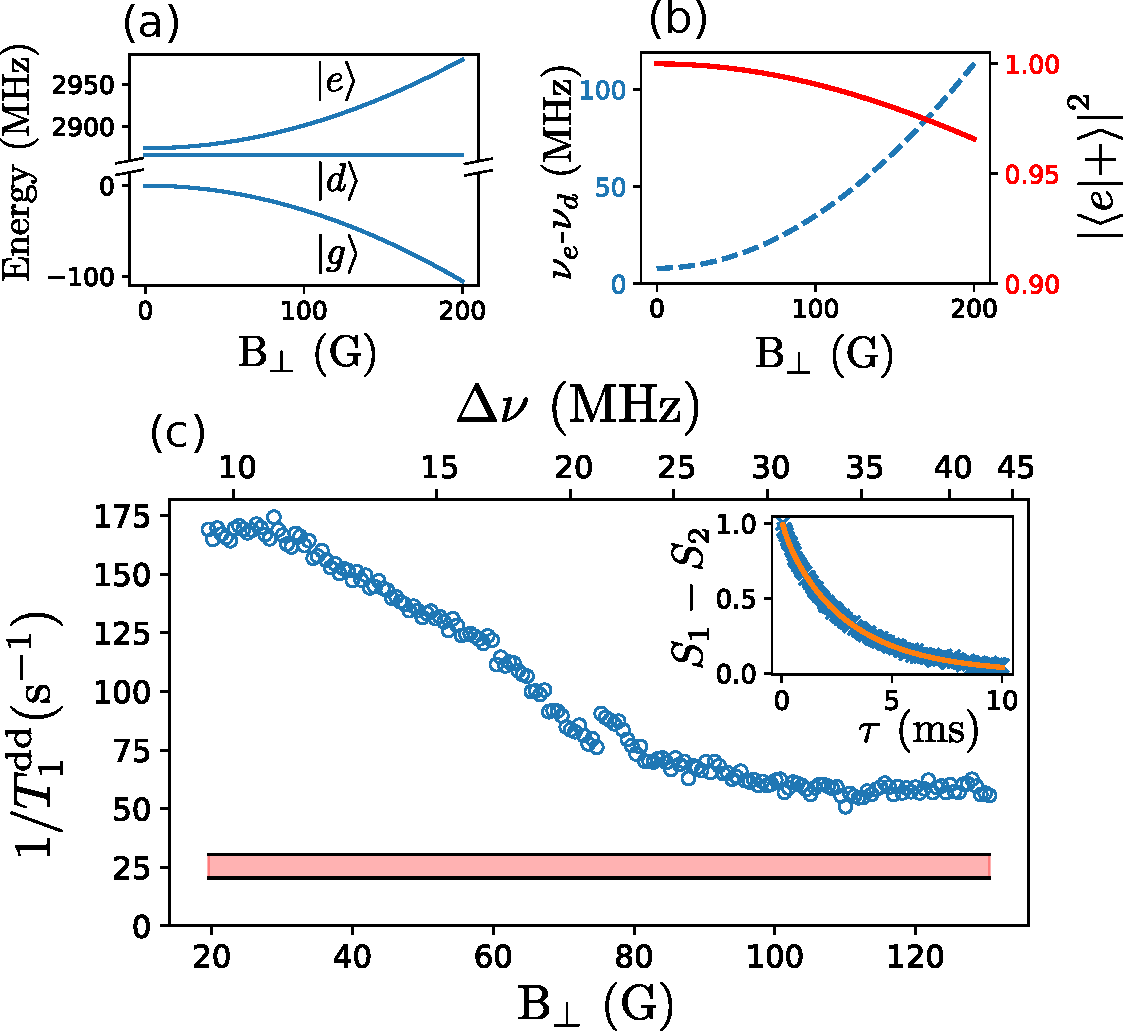
\includegraphics[width=0.45\textwidth]{Figures/fig_transverse_field_V2.pdf}
\caption{(a) Energies for the spin Hamiltonian in the presence of pure transverse magnetic field $B_\perp$. The three spin levels are denoted $\ket{g}$, $\ket{d}$ and $\ket{e}$. (b) Blue dashed curve : frequency detuning $\Delta \nu$ between the $\ket{e}$ and $\ket{d}$ states. Red plain curve : Matching factor $\abs{\bra{e}\ket{+}}^2$ between the states $\ket{e}$ and $\ket{+}$. (c) Measurement of the stretched exponential decay rate $1/T_1^{\rm dd}$ for a single class of sample HPHT-150-2 as a function of the amplitude of a purely transverse magnetic field. The red dashed line corresponds to the plateau reached for high transverse field. The green dashed line correspond to the value found for the same sample with a longitudinal magnetic field, with error bars. The corresponding detuning between the states $\ket{d}$ and $\ket{e}$ is indicated on top.}
\label{B_transverse}
\end{figure}
Similarly, we compute the predicted decay rate when $\bm B \parallel \left[100\right]$ case compared when $\bm B = 0$, and find a theoretical increase of $\sim 20\%$ when $\bm B = 0$ due to the mixing by the local electric field. This, along with the double-flip processes explains the behavior observed in Fig. \ref{100_VS_1x4} (c)-ii) and (c)-iii).

%... (lis un peu ce que t'as déja écrit avant de tout réécrire, je te connais moi futur. En vrai c'est de la merde, j'ai tout réécrit)
%The dipole-dipole interaction Hamiltonian between two spins ${\vec S}_1$ and ${\vec S}_2$ reads :
%\begin{equation}
%\mathcal{H}^{\rm dd}= -\frac{J_0}{r^3}\left(3\left({\vec S}_1 \cdot \vec u \right)\left({\vec S}_2 \cdot \vec u \right) - {\vec S}_1 \cdot {\vec S}_2  \right),
%\end{equation}
%Where $J_0= (2 \pi) 52\ \rm MHz \cdot \rm{nm}^3$, $\vec r$ is the relative positions of the two spins and $\vec u = \frac{\vec r}{\norm{\vec r}}$. In situations such as the one described in Fig. \ref{largeur_fluct}, the only relevant terms of $\mathcal{H}^{\rm dd}$ in term of population transfer are the flip-flop terms such as $\mel{0,+1}{\mathcal{H}^{\rm dd}}{+1,0}$. In zero magnetic field however, we have to take into account other aspects of the dipolar Hamiltonian in consideration.
%
%First is the change of basis of the single spin Hamiltonian $\mathcal{H}_s$ : in zero external magnetic field, the eigenstates of $\mathcal{H}_s$ in the $\{\ket{+1},\ket{-1}\}$ manifold are determined by local electric and magnetic field coming from nearby impurities \cite{mittiga2018imaging}. For the samples used in this study, $\mathcal{H}_s$ was dominated by local electric field (see SI), meaning that the proper eigenstates of $\mathcal{H}_s$ in zero magnetic field are $\{ \ket{0},\ket{+}=\frac{\ket{+1}+\ket{-1}}{\sqrt{2}},\ket{-}=\frac{\ket{+1}-\ket{-1}}{\sqrt{2}} \} $%
%Because the splitting between $\ket{+}$ and $\ket{-}$ ($\approx 9\ \rm MHz$) is much greater than the dipole-dipole interaction ($J_0 / r^3 \approx 30\ \rm kHz$), the flip-flop terms of $\mathcal{H}^{\rm dd}$ now reads $\mel{0,+}{\mathcal{H}^{\rm dd}}{+,0}$. Averaging over all relative positions of two aligned NV centers, we found that on average $\abs{\mel{0,+}{\mathcal{H}^{\rm dd}}{+,0}}$ was greater than 
%$\abs{\mel{0,+1}{\mathcal{H}^{\rm dd}}{+1,0}}$ by a factor $1.8 \sim 2$ depending on the correlation lengths of the local electric field.
%When all four classes are resonant, the theoretical decrease in the spin lifetime due to the change of basis is $\sim 20 \%$ (See SI de ouf).
%
%Second is the near-resonance condition of the double-flip processes such as $\mel{0,+1}{\mathcal{H}^{\rm dd}}{-1,0}$ or $\mel{0,+}{\mathcal{H}^{\rm dd}}{-,0}$. These terms usually couple non resonant states due to the energy mismatch between $\ket{+1}$ and $\ket{-1}$. However in zero field, the energy splitting between $\ket{+}$ and $\ket{-}$ is comparable with the fluctuator's spectral width measured in Fig. \ref{largeur_fluct} to be $\approx 8\ \rm MHz$, making the double-flip population transfer possible.
%
%\begin{figure}
%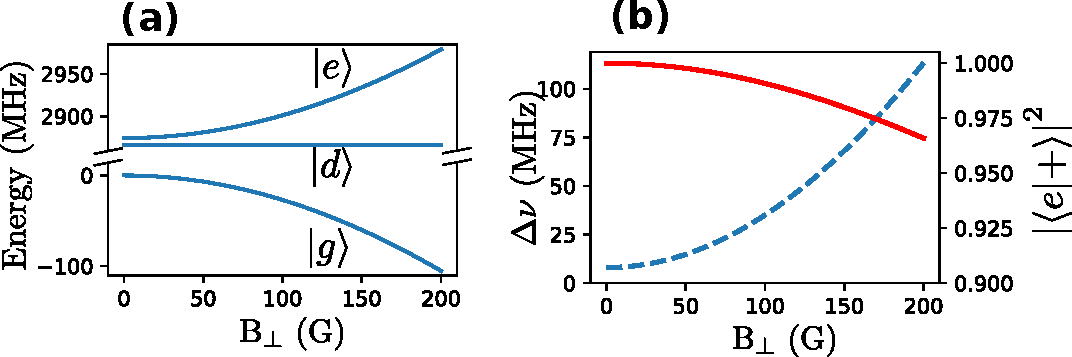
\includegraphics[width=0.45\textwidth]{Figures/fig transverse field simu}
%\caption{Simulated eigenstates of the spin Hamiltonian in the presence of purely transverse magnetic field. (a) Energies of the three eigenstates $\ket{g}$, $\ket{d}$ and $\ket{e}$ as a function of the magnetic field amplitude. (b) Blue dashed curve : frequency detuning between the two transitions $\ket{g} \leftrightarrow \ket{d}$ and $\ket{g} \leftrightarrow \ket{e}$. Plain red curve : projection of $\ket{e}$ on $\ket{+}=(\ket{+1}+\ket{-1})/\sqrt{2}$ as a function the magnetic field. Is equal to the projection of $\ket{g}$ on $\ket{0}$.}
%\label{calculs_B_transverse}
%\end{figure}
%
%In order to evaluate the relative contribution of these two factors, we investigate the spin relaxation in the case of pure transverse magnetic field. Calling $\{ \ket{g}, \ket{d}, \ket{e} \}$ the three eigenstates of the spin Hamiltonian in the presence of purely transverse magnetic field, Fig. \ref{calculs_B_transverse} shows that for small enough magnetic field, the $\{ \ket{g}, \ket{d}, \ket{e} \}$ basis is almost equal to the $\{ \ket{0},\ket{+},\ket{-} \} $ basis : for $B=120\ \rm G$, $\braket{0}{g}\approx 0.99$, $\braket{-}{d}=1$ and $\braket{+}{e}\approx 0.99$. However the energy difference between $\ket{d}$ and $\ket{e}$ reaches $\approx 45\ \rm G$ which is high enough to cancel out the double-flip processes and allows us to isolate the change of basis hypothesis from the double-flip one.
%%As shown in Fig. SOON, (and in SI), the $\{ \ket{0},\ket{+},\ket{-} \} $ basis correspond to the spin Hamiltonian eigenstates in two situations : either in zero magnetic field when the electric field dominates, or when the magnetic field is purely transverse, as long as it remains small before the zero-field splitting. %(rq : est-ce que je dois mettre le hamiltonien de spin dans le main text du coup ?).
%
%\begin{figure}
%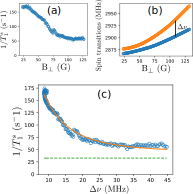
\includegraphics[width=0.45\textwidth]{Figures/fig transverse field}
%\caption{Modification of the stretch lifetime in the presence of purely transverse magnetic field. (a) Stretch component of the ensemble lifetime as a function of the field amplitude. (b) Transition frequencies for the $\ket{g} \leftrightarrow \ket{d}$ and $\ket{g} \leftrightarrow \ket{e}$ transitions, measured through ODMR. (c) Stretch component of the lifetime as a function of the frequency detuning between the two transistions (blue circles), fitted by a Lorentzian centered in $\Delta \nu=0$ with half width at half maximum 8MHz. The green dashed line correspond to the lifetime of a single class aligned with the magnetic field.}
%\label{exp_B_transverse}
%\end{figure}
%
%Fig. \ref{exp_B_transverse} shows the dipole-dipole spin relaxation $T_1^{\rm dd}$ for a class of NV whose axis is orthogonal to the applied magnetic field. By monitoring the frequencies of the transitions $\ket{g} \leftrightarrow \ket{d}$ and $\ket{g} \leftrightarrow \ket{e}$, we can deduce the detuning $\Delta \nu$ between the two-spin states $\ket{0,+}$ and $\ket{-,0}$. Plotting then $1/T_1^{\rm dd}$ as a function of $\Delta \nu$, we can notice two things. 
%
%First the decrease of $1/T_1^{\rm dd}$ as $\Delta \nu$ increases which corresponds to the loss in effectiveness of the double flip processes. The shape of the curve matches decently well with the tail of a Lorentzian centered in $\Delta \nu=0$ with a width of 8 MHz, confirming that the double-flip process interaction range is likely determined by the fluctuators noise spectrum just like the flip-flop processes. 
%
%Second is the plateau reached for $\Delta \nu \gtrsim 30\ \rm MHz$. The final $1/T_1^{\rm dd}$ value is about twice as high as that for a spin well aligned with the magnetic field, showing the increased depolarization due to the change of basis.
%
%This experiment shows that, for the sample studied here, the depolarization due to the double-flip processes dominates the one due to the change of basis in zero magnetic field.

\begin{figure}
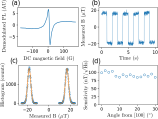
\includegraphics[width=0.45\textwidth]{Figures/fig_magneto}
\caption{Low field magnetometry protocol. (a) Demodulated photoluminescence as a function of an externally applied magnetic field with an additional oscillatory magnetic field. (b) Measured magnetic field when alternating a small external magnetic field offset. (c) Histogram of the measurement in Fig. (b) fitted with gaussians of standard deviation $\sigma=1.5\ \mu \rm T$. (d) Measured sensitivity as function of the angle between the external magnetic field and the [100] crystalline axis.}
\label{magneto}
\end{figure}
%

Our observations have important implications for magnetometry with NV ensembles.
DC microwave-free magnetometry has already been performed using either NV-NV cross-relaxations \citep{akhmedzhanov_microwave-free_2017,akhmedzhanov_magnetometry_2019} or level anti-crossing \citep{Wickenbrock, zheng2017level, zheng_microwave-free_2020}. Here we propose to perform a similar protocol , but using the spin depolarization at zero-field as proposed in \cite{filimonenko2018weak, filimonenko2022manifestation}. The main advantage with the previously mentioned protocols is the fact that the sensitivity does not depend crucially on crystalline orientation, making this protocol applicable with diamond powders or polycrystalline samples. 

Fig. \ref{magneto} (a) shows the demodulated PL as a DC magnetic field is scanned in a random direction and an additional alternating magnetic field of amplitude $\sim 10\ \rm G$ and frequency  $\sim 1\ \rm kHz$ is added through the same electromagnet. The sample used here is HPHT-15-1 and the laser power $\sim 1\ \rm mW$.  We can see a sharp linear slope in low field $\abs{B} < 5\ \rm G$. Once calibrated, in this case with ODMR, the slope can provide a 1D magnetic field measurement, which could be extended to 3D with a set of 3 coils or 3 electromagnets, as in \cite{zheng_microwave-free_2020}. In order to assess the sensitivity of the measurement, we alternate a small DC field of $\approx 40\ \mu\rm{T}$ every few seconds and take a histogram of the measured fields, as shown in Fig. \ref{magneto} (b) and (c). The histogram is well fitted with gaussians of standard deviation $\sigma=1.5\ \mu \rm T$. The measurement was performed here with an output low-pass filter of time constant $\tau=3\ \rm ms$, which gives us a sensitivity $\eta=\sigma \sqrt{\tau}=82\ \rm{nT}/\sqrt{\rm Hz}$.

We now evaluate the relative role of the three causes of spin depolarization in the magnetometer, namely the splitting of the classes, the local electric field and the double-flip processes. In order to do so, we measure the magnetometer sensitivity while changing the angle of the magnetic field.  The results are shown in Fig. \ref{magneto} (d). We can see a slight increase of $\sim$ 10\% in the sensitivity as we leave the [100] region, but overall the sensitivity remains relatively flat. 
When $\bm B$ is aligned with the [100] crystalline axis, only the double flips and the electric field cause a depolarization, whereas in every other orientation the three effects are at play.
The double-flips and electric field effects are thus the dominant factors in the sensitivity of this protocol. While it may seem surprising that the effects with a lower contribution on the PL contrast have a higher effect on this PL-based protocol, what matters here is not the absolute contrast but the slope of the change of contrast with respect to the magnetic field. The latter is in fact larger for the local electric field and double flips processes than for the process involving only flip-flops. 
%This is in agreement with the measurements in Fig. \ref{100_VS_1x4} : even though the contrast is much better in the not-[100] case, the slope in term of contrast percentage/magnetic field is comparable in both cases (en faite pas complètement, y'a pas loin d'un facteur 2 sur les dérivées numériques)
It should be noted that this observation is sample dependent, and that other samples, including from the same batch, have shown a higher orientation dependence, corresponding to a lower contribution from the electric field and double-flip processes.

As a conclusion, we identified three mechanisms causing extra spin depolarization in zero field for dense ensemble of NV$^-$ centers, all related to an increase in the dipole-dipole induced cross-relaxations between the spins of NV centers. The lift in degeneracy of the spin state of different NV classes was found to be the main cause of zero-field depolarization, followed by double-flip processes and then the electric field induced mixing. We have employed cross-relaxation for microwave and orientation-free DC-magnetometry and demonstrated a sensitivity below $100\ \rm{nm}/\sqrt{\rm Hz}$ for a single $10\ \mu \rm m$ commercially available diamond and show that that double-flips and electric field play an important role.
Besides magnetometry, our work offers prospects for understanding many body phenomena with strongly coupled spins. 
%DEER, many body, critical thermalization, 2D. Double quantum 

\section*{acknowledgements}

\bibliographystyle{plain}
\bibliography{CR}{}



\end{document}